\documentclass[chapterprefix=false]{scrreprt}
%Gummi|065|=)

\usepackage{blindtext}
\usepackage[T1]{fontenc}
\usepackage[utf8]{inputenc}
\usepackage{tabularx}
\usepackage{array}
\usepackage{float}
\usepackage{longtable}
\usepackage{booktabs}
\usepackage{graphicx}
\usepackage{rotating}
\usepackage{cite}

\setlength{\parskip}{1em}
\setlength{\parindent}{0em}

\graphicspath{ {./images/} }
\restylefloat{table}

\title{Interim Report \\
  Domain Specific Language \\
  for Social Media Bots}
    
\author{Samuel Withey \\
	Supervisor: Ian Wakeman}
	
\date{}

\begin{document}

\maketitle

\newpage

\tableofcontents

\newpage

\renewcommand{\chaptername}{} 

\chapter{Interim-Report}

\section{Introduction}

In January 2019, according to Hootsuite's digital report, there were 3.484 billion worldwide active users across all social media platforms \cite{global-digital-report-2019}. This rapid social paradigm shift has transformed consumer behaviour and social interaction through online social platforms which allow instantaneous direct communication. This has provided unbounded limitations for brands to connect and engage directly with their audiences.

\subsection{Goals, Aims and Objectives}

The overall goal of this project is to provide a solution to the issues around managing social media content. This solution will be achieved by providing tools to automate managing and posting content on social media platforms. The aims for these tools are to allow the user to post content for a single account on multiple social media platforms at once, schedule these posts and automate replies and direct messages to other users on the platforms.

The solution for the project can be split into three main objectives. The first objective is to design a system or tool to provide the user with methods to automate the features and capabilities of what can be done by a user on social media platforms. The second objective is to design a system or tool to execute these features and capabilities of the first objective and the third objective is to design a centralised system to display customisable feeds for multiple social media platforms.

\subsection{Problem Area}

The first objective will be achieved by designing and implementing a domain specific language and parser to be able to configure and automate the features on social media platforms. The second objective will be achieved by implementing an interpreter to translate the domain specific language into executable pre-compiled code to interact with the social media platforms. The third objective will be achieved by implementing a web application which displays customisable feeds for multiple social media accounts in a centralised interface.

Domain specific languages are optimised for a given class of problems called a domain.  It is based on abstractions that are closely aligned with the domain for which the language is built and a domain specific languages syntax is suitable for expressing these abstractions concisely. This differs from general-purpose languages which are used by programmers to instruct computers. General-purpose languages are Turing complete, which means they can be used to implement anything that is computable by a Turing machine.\cite{DslEngineering2013}

An advantage of using a domain specific language is that it is another layer of abstraction. Notation can be defined that expresses the abstractions concisely and makes interacting with programs easy and efficient. This is important for the project as the domain specific language can be used by non-programmers. It provides a clean level of abstraction that moves away from general-purpose languages and API’s which non-programmers are not competent enough to use and allows them to work with a language closely aligned with the domain they work in \cite{DslEngineering2013}. This is a key solution to the problem area as it abstracts the complexity of using API’s by creating a language which is syntactically simpler than a general purpose language and can be used by non-programmers which is the target user for the system.

For the domain specific language to execute it requires an interpreter or compiler. When text is interpreted, it is parsed and the result from the program is produced in a single process. 

\begin{center}
 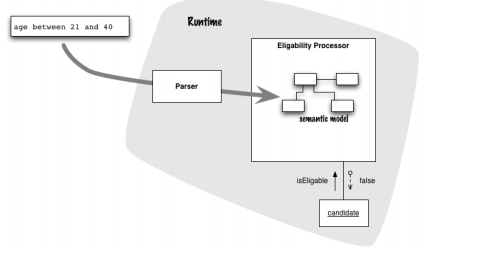
\includegraphics[scale=0.7]{interpreter}
 \newline
 \caption{Interpreter parsing text and produces result \cite{DBLP:books/daglib/0034522}}
\end{center}

A parser is the processing of structuring a text according to a given grammar. The parser will generate a syntax/parse tree which is a data structure which precisely shows how various segments of the program text are to be viewed in terms of the grammar. A grammar or context-free grammar are the formalism for describing the structure of programs in a programming language by describing the syntactic structure. Since the semantics of a language is defined in terms of the syntax, the context-free-grammar is also instrumental in the definition of the semantics\cite{grune2012modern}.

\begin{center}
 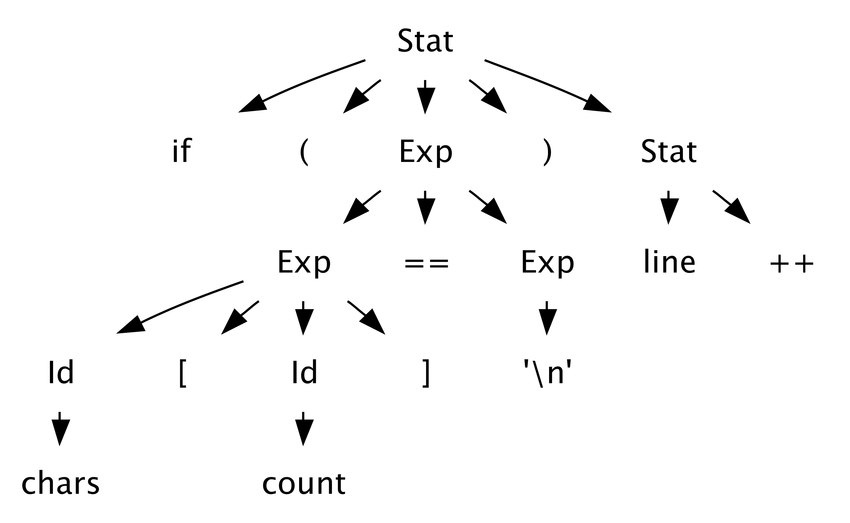
\includegraphics[scale=0.4]{parse-tree-java}
 \newline
 \caption{Java Parse Tree \cite{java-parse-tree}}
\end{center}

The alternative to interpretation is compilation. Compilation parses a program text and produces an intermediate output, which is then separately processed to provide desired behaviour. For domain specific languages the compilation is often referred to as code generation. An advantage of code generation is that code can be generated in any programming language. This is useful for the project as the code generated would interact with the API for the social media platforms\cite{DBLP:books/daglib/0034522}.

\begin{center}
 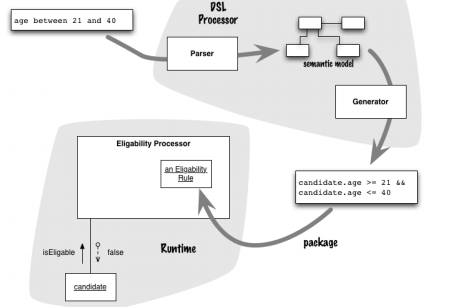
\includegraphics[scale=0.7]{compiler}
 \newline
 \caption{Compiler parsing text \cite{DBLP:books/daglib/0034522}}
\end{center}

A state machine is a model of a system as a set of explicit states with transitions between them. Internal states can be classified and the system can move between states depending on some internal property and event; thus a sequence of events leads from state to state\cite{DBLP:books/daglib/0034522}.

\begin{center}
 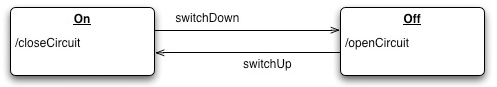
\includegraphics[scale=0.7]{state-machine}
  \newline
  \caption{State Machine \cite{DBLP:books/daglib/0034522}}
\end{center}

A semantic model is a state machine which captures the legal expressions of a program and the model defines the semantics. For a semantic model to work, the domain specific language provides a readable way of populating the model and acts as a mechanism for how the model is configured\cite{DBLP:books/daglib/0034522}.

\begin{center}
 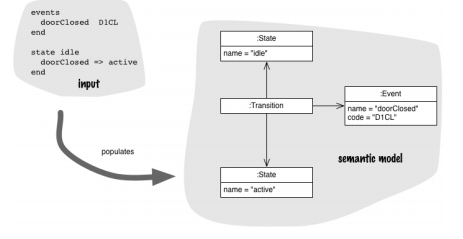
\includegraphics[scale=0.7]{dsl-semantic-model}
  \newline
  \caption{Parsing DSL populates semantic model \cite{DBLP:books/daglib/0034522}}
\end{center}

Semantic models can be implemented into the compilation stage which allows the separation of the parsing, execution semantics and the code generation. An advantage of using semantic models is the interpreter and code generation can both be completed from the same semantic model which makes the process simpler. The domain specific language acts as a front-end to the semantic model which provides a different style of manipulation to the command-query API\cite{DBLP:books/daglib/0034522}.

\subsection{Motivation}

The motivation for this project was to provide a unique solution for social media automation and management. The project scope covers multiple compelling areas within computing such as compilers and interpreters, software engineering, web applications and distributed systems. Other motivations for the project includes the opportunity to use industry standard tools and applications such as parser generators, application programming interfaces, version control systems, web frameworks and cloud computing services.

The project was inspired by previous industry experience working for a large tech company which provided tools to solve issues around paid advertisement. This inspiration led to a desire to explore unique solutions to manage and automate organic social media content and interactions for multiple social media platforms simultaneously. Other industry experience working on intricate web applications inspired the projects social media management tool to be created using Pythons Web Framework Django. 

The ultimate motivation for the project is to apply and continue to develop the skills learnt in previous job roles and at higher education into compelling areas of computing for future graduate job roles.


\subsection{Relevance}

The project relevance extends to various areas in computing that have been studied at higher education and have been applied in prior work experience. The main area in computing that this project explores is the domain specific language and interpreter. This area of computing has been previously taught through Compilers and Computer Architecture module at University. This is an important research topic within Computer Science and will be useful to apply the knowledge from this subject area to a practical application.

Another area of computing that this project explores is Software Engineering. This subject area is relevant to the project as the domain specific language will require rigorous design to ensure that it is scalable, efficient and usable and will require more traditional waterfall planning and techniques. The development of the domain specific language, interpreter and web application will be completed using an Agile/Scrum methodology. Both design and development techniques were initially taught in the Software Engineering module and are widely used in the industry today.

The programming for the project will predominantly be completed using Python 3. According to GitHub’s Octoverse Report, Python outranked Java as the second most popular language on GitHub by repository contributors\cite{github}. Python is one of the most popular programming languages and is a useful skill to develop for this undergraduate course and future job opportunities. Using API’s, frameworks and hosting web applications on cloud services will be useful practical skills for future job opportunities and education.


\newpage

\section{Professional Considerations}

The nature of the project using social media automation results in multiple different ethical issues and considerations. The intent of the project is to allow more automation and control across social media content for brands and businesses to engage with their audience, however social media automation can be used for many other reasons and this leads to many ethical considerations and consequences. Examples of real world negative ethical consequences of social media automation are spam, harassment, spreading false information, troll armies and influencing content reach and impressions.

\subsection{US Presidential Election 2016}

One of the most infamous incidents in which Twitter and Facebook bots have been used in recent years is the role the bots took in the United States 2016 presidential election\cite{us-election}. Twitter bots were claimed to be configured to interact with certain political figures. This was done to give these tweets more exposure, boost their ranking on Twitter's trending page, manipulate traffic and spread false information. This incident has been referred to as a threat to democracy and Twitter has received increasing pressure to deactivate and restrict bot accounts \cite{gorbis_woolley_2019}. It is estimated that nearly 48 million Twitter accounts are operated by bots, with 15\% of the total accounts coming from automated bots\cite{varol2017online}. The use of bots to spam content and engage with certain accounts is prevalent across all social media platforms and is a growing trend.

\subsection{BCS Code of Conduct}

The project will adhere to all BCS code of conduct standards. With the nature of the project and ethical issues discussed, Section 1 Public Interest is an import standard. It is important to have regard for public health, privacy and security and I shall achieve this in the project by directly implementing API limitations and rules from the platform. This will help with public health as restrictions will be placed on the frequency of posts to reduce spam, trolling and harassment.

Another important standard is Section 2 Professional Competence and Integrity. Section 2(c) is important to my project as the system will be designed for practical application. The system will be designed to comply with all current technological developments and procedures. Section 2(d) is important as the project will be used in practice. Legislation such as GDPR will be important to the project as the wider scope of the project is to include analytics. I will comply with GDPR legislation around data processing, data handling and anonymizing data.

The project aims to involve human participants for usability testing of the system. This would require an approved ethical review and a Ethical Compliance Form will be submitted in the near future. This is to comply with Section 3(a) to carry out professional responsibilities with due care and diligence in accordance with the relevant Authority’s requirements. 

\newpage

\section{Related Work}

\subsection{TweetDeck}

TweetDeck is a social media dashboard application for Twitter and is integrated into Twitter’s interface. The application interfaces with the Twitter API to allow users to send and receive tweets and view profiles\cite{tweetdeck}. 

TweetDeck consists of a series of customisable columns which can be customised to display:

\begin{itemize}
 \setlength\itemsep{-0.75em}
 \item Home: Home timeline for any specific account.
 \item User: Tweets from a specific account.
 \item Notifications: Notifications for a specific account, including when the account's Tweets are Retweeted, liked, or mentioned, and when someone follows the account.
 \item Search: A specific search term.
 \item Lists: Create or connect a list you already follow.
 \item Collection: A timeline of curated Tweets, hand-selected by you, to share with others.
 \item Activity: What’s happening with the accounts you follow.
 \item Likes: Tweets marked as likes from a specific account.
 \item Messages (one account): Direct Messages for a specific account.
 \item Mentions (one account): When someone mentions a specific account.
 \item Followers: Follow activity for a specific account.
 \item Scheduled: Your scheduled Tweets.
 \item Messages (all accounts): Direct Messages from all your authorized accounts in aggregate.
 \item Mentions (all accounts): Mentions from all accounts.
 \item Trending: Specific worldwide trends.
\end{itemize}

\begin{center}
 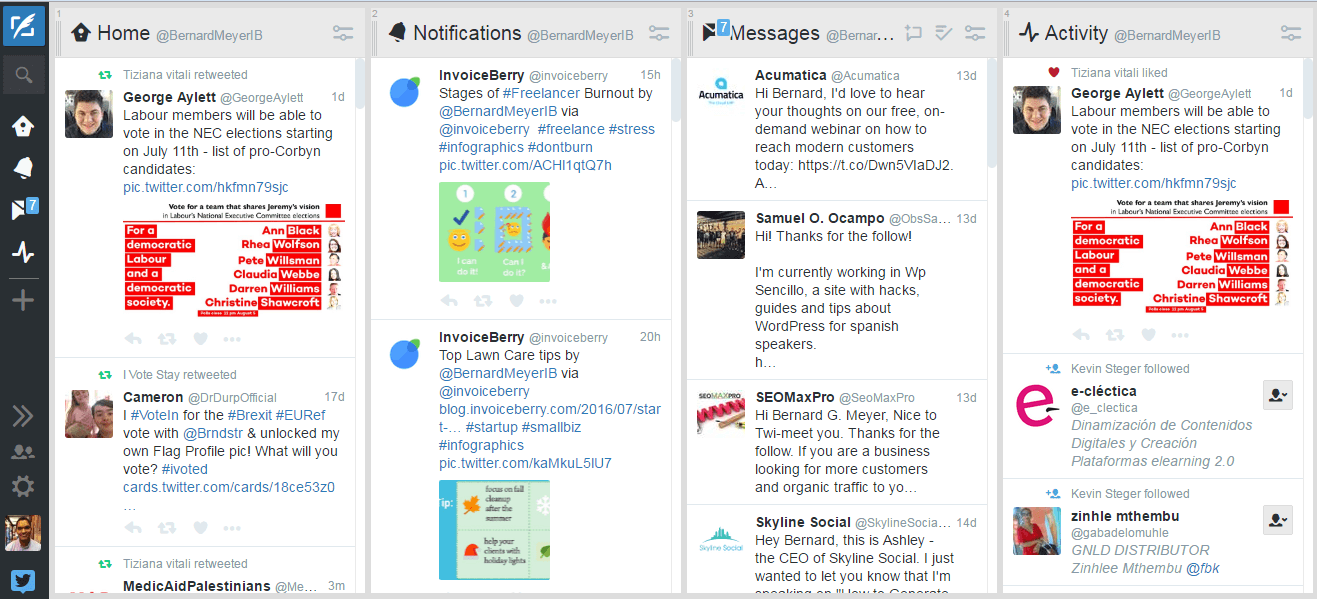
\includegraphics[scale=0.3]{tweetdeck-screenshot}
 \newline
 \caption{TweetDeck Dashboard \cite{tweetdeck-dashboard}}
\end{center}

TweetDesk has advanced features for consuming and analysing lots of information at once. TweetDesk supports advanced features such as Tweet Scheduling, collections, search, filtering and more \cite{tweetdeck-features}. 

\begin{itemize}
 \setlength\itemsep{-0.75em}
 \item Scheduling: TweetDeck allows users to schedule Tweets in advance.
 \item Collections: Collections are organised Tweets according to topics, events, interests,  and conversations all in real time and can be added as columns.
 \item Advanced search: TweetDeck runs real-time search including sentiment.
 \item List Management: TweetDeck allows users to manage lists in one centralised place for multiple accounts. Lists can be created by filtering interests or by particular accounts.
 \item Embedded Tweets: TweetDeck can create embedded Tweets directly from the app.
\end{itemize}

\subsection{Hootsuite}

Hootsuite is a social media management tool which manages over 35 popular social networks in one place. The system's user interface takes the form of a dashboard to monitor multiple streams in one place \cite{inc._2019}.

\begin{center}
 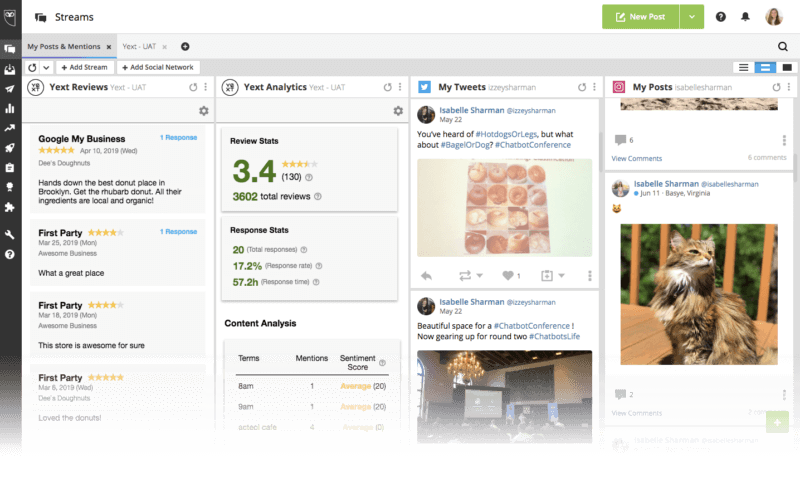
\includegraphics[scale=0.5]{hootsuite-dashboard}
 \newline
 \caption{Hootsuite Dashboard \cite{gesenhues_gesenhues_2019}}
\end{center}

Core features of the Hootsuite platform include:

\begin{itemize}
 \setlength\itemsep{-0.75em}
 \item Scheduling
 \item Content Curation
 \item Promoting
 \item Analytics
 \item Monitoring
 \item Team Management
 \item Security
 \item Apps and Integration's
\end{itemize}

Hootsuite provides other products:

\begin{itemize}
 \setlength\itemsep{-0.75em}
 \item Amplify: Allows staff to share company news
 \item Insights: Presents data in real-time through visual reports
 \item Impact: Generates ROI for marketing campaigns
 \item Ads: Platform for social advertisement
\end{itemize}

\subsection{Social Bot}

Social bot is a project stored in a public repository on GitHub. The project description in the README is Python bots for social networks. The project supports Twitter, Instagram \& Facebook. This project provides most functionality for Twitter, as it can post, reply, retweet, quote and like tweets. It can also follow \& unfollow users, get users and tweets by a term search and get user profile details. Instagram and Facebook bots are more limited for this project as they cannot post or schedule and can only retrieve user data and posts. The API provides granular action-functions that can be used by bots operating individually or as swarm \cite{socialbot}.

\subsection{Software Bots}

Software Bots is a report published by IEEE which explores the types of bots, platforms for working with bots and offers guidelines on how to create and use them. 

According to the report, bots can be categorised through their interaction model. Some bots support a domain-specific language in which users interact with bots using specific commands in a command line interface while other bots might parse natural language through text or speech. Other bots can also include UI controls that lets users respond and interact quickly. Bots can be characterised according to their purpose:

\begin{itemize}
 \setlength\itemsep{-0.75em}
 \item Generalist bots such as Siri or Cortana support a range of simple tasks and direct users to appropriate external resources when deeper knowledge is required. 
 \item Transactional bots work on the users’ behalf, automatically executing transactions with external systems (for example, automatically making a purchase when a price level is reached).
 \item Informational bots fetch information for users (for example, gathering insights about stocks or providing weather updates).
 \item Productivity bots improve user or team productivity by automating rote or tedious tasks (for example, updating calendars or silencing notifications).
 \item Collaboration bots help users communicate, coordinate, and collaborate
\end{itemize}

There are multiple tools for bot development and these tools are distinguished for building bots (creation platforms) and the platforms on which the bots dwell (distribution platforms). Creation platforms provide a variety of software foundations, frameworks, tool-kits, APIs and other features. These provided services range from well documented code templates to out the box no-code required bot-building interfaces. Distribution platforms dictate where and how users access bots and many focus on social networking and messaging. 

With the increase in popularity of bots and the significant role they play in day-to-day life it is important to understand what works well and what does not. Users should always know what to expect and bot developers should make it clear to users that they are interacting with a bot. User-bot interaction should be a smooth and frictionless experience and bots should do no harm. Developers should carefully consider how their bots could be misused intentionally or unintentionally. Many bots are already deemed malicious so building user trust poses challenges\cite{8239928}.

\subsection{Research}

The background research for the related work includes two industry standard social media management tools, an online repository for social media bots and a report around the current state of software bots. There was limited background research for domain specific languages for software bots as it is not a well researched topic and social media management tools do not have open source code. Research was therefore conducted on indstry tools such as TweetDeck and Hootsuite, an example of a social media bot and a published report on all aspects of Software Bots. 

This research was important as TweetDeck demonstrates all the functionality of a web application solely using the Twitter API. This application is similar to the overall scope of the project however the project aims to provide a similar application across multiple platforms. Hootsuite is an all in one robust social media management tool. It provides methods of high level abstraction from interacting with the social media platforms API through a drag and drop centeralised dashboard. Hootsuite is similar towards the overall goals of the project however the project aims to abstract the interaction of the API's through a domain specific language and separate the web application from this. Hootsuite includes streamlining team management and integrated analytics which is outside the scope of the project.

Social Bot demonstrates the functionality of social media bots using the API's in a command-line interface. This is important to the project as it demonstrates what can be achieved using a different approach. Software bots presents information about the different types of bots, categorising these bots, how the bots work and what platforms they work on and solutions to ethical implications bots pose. This was useful initial research as it allowed direction for the project and helped with the content of the interim report.

\newpage

\section{Requirements Analysis}

The system is aimed to be directed towards general users, brands and agencies who use social media daily to connect with their audiences. It is vital to understand the needs of this audience, to what extent current solutions meet their needs and what else they would like to see from current solutions. To help understand this, an interview was conducted with InCrowd.

InCrowd is a company based in London and Brighton who provide intuitive sports technology to help brands engage with their audiences. The interviewees who work for InCrowd are Matt and Helen, who work in the Marketing team for InCrowd. Matt works with SkyBet and solely uses Twitter and native Twitter tools in his day to day job role. Helen works in the Business to Business (B2B) marketing team and focuses on using Twitter and Linkedin to achieve this role. Both interviewees use the native platforms tools and applications but have used other industry standard social media management tools to automate and schedule content in previous job roles.

To understand InCrowds needs, functional and non-functional requirements are produced to identify their needs and provide scope on the overall direction of the project. The requirements analysis has been completed from the interview that was conducted with InCrowd. InCrowd provided ethical consent to use selected quotes from the interview in the report and this is included in the appendix. Further requirements have been extracted from related work as some features are essential for the project. The project is designed to meet InCrowds needs however it has been designed with the intention to be used by any brand or agency and not exclusively for InCrowd.

\subsection{Functional Requirements}

\newcolumntype{P}[1]{>{\arraybackslash}p{#1}}
\newcolumntype{C}[1]{>{\centering\arraybackslash}m{#1}}

\begin{longtable}{|>{\centering}C{1.7cm}|P{7cm}|C{3.7cm}|} \hline
    {Reference} & {Description} & {Mandatory/Desirable} \\ \hline
    F1 & The system shall provide the basic functionality of what actions can be completed by a human on Twitter which can be configured by the domain specific language. This functionality includes login, post tweets, reply to tweets, retweet tweets, like tweets and follow users. & Mandatory \\ \hline 
    F2 & The system shall provide the basic functionality of what actions can be completed by a human on Instagram which can be configured by the domain specific language. This includes getting an Instagram profile and getting an Instagram user's images, video's and albums. & Mandatory \\ \hline
    F3 & The system shall provide the basic functionality of what actions can be completed by a human on Facebook which can be configured by the domain specific language. This functionality includes posts, reading notifications and messages. & Mandatory \\ \hline
    F4 & The system shall allow simultaneous scheduling for content across Twitter, Instagram and Facebook. & Mandatory \\ \hline 
    F5 & The system shall provide the ability to have a different content set optimised for each social media platform in the same content schedule. & Mandatory \\ \hline
    F6 & The system should provide a web interface as a single dashboard for different feeds. & Mandatory \\ \hline
    F7 & The web interface shall be similar to Tweetdeck's UI having multiple columns. & Mandatory \\ \hline
    F8 & The system shall provide customisable columns for multiple social media platforms for F7. & Mandatory \\ \hline
    F9 & The system shall provide the functionality of personalised automated support responses for directing messaging on Twitter and Facebook. & Mandatory \\ \hline
    F10 & The system should retrieve a list of relevant content from other users on the platform based on a customisable input such as keywords and hashtags. & Desirable \\ \hline
    F11 & The system shall provide the ability to remove content from the list provided in F10 and provide the ability to interact with the content with the use of a single click. & Desirable \\ \hline
    F13 & The system should have a central messaging system which provides the functionality of directly message users across multiple platforms in one inbox. & Desirable \\ \hline
    F14 & The system should provide a list of suggested accounts to follow based on inputs such as keywords and hashtags. & Desirable \\ \hline
    F15 & The system should provide a list of people who engage with the accounts the most in a given time frame. & Desirable \\ \hline
    F16 & The system should provide the ability to customise reports within a given timeframe. & Desirable \\ \hline
    F17 & The system should be integrated into InCrowd’s native insights tool Bridge. & Desirable \\ \hline
\end{longtable}
    
\subsection{Non-Functional Requirements}

\begin{longtable}{|>{\centering}C{1.7cm}|P{7cm}|C{3.7cm}|}  \hline
    {Reference} & {Description} & {Mandatory/Desirable} \\ \hline
    NF1 & The domain specific language shall run on Windows, Mac and Linux Operating Systems. & Mandatory \\ \hline
    NF2 & The domain specific language shall be programmed using Python 3 and use ANTLR 4 toolkit. & Mandatory \\ \hline
    NF3 & The interpreter shall run on Windows, Mac and Linux Operating Systems. & Mandatory \\ \hline
    NF4 & The interpreter shall be programmed using Python 3. & Mandatory \\ \hline
    NF5 & The web application shall run on all latest browsers. & Mandatory \\ \hline
    NF6 & The web application shall be programmed using Python 3 and Django Web Framework. & Mandatory \\ \hline
    NF7 & The web application shall use Django's user login system to provide security for the web application through user authentication. & Mandatory \\ \hline
\end{longtable}

\subsection{Requirements}

The ideal system for InCrowd would be a social media management system which allows scheduling and automated content across all platforms integrated into their proprietary insights system. The project aims to contribute to their needs by providing a domain specific language to automate and schedule content and provide a customisable web interface to act as a social media management system. The project will not be able to be integrated into their proprietary insights system.

The automation and scheduling of content and web application is expected to be completed within the given time frame. The goal is to complete all mandatory requirements and as many desirable requirements as possible however some of the desirable requirements are intricate tasks which may not be completed within the time frame. The project will be designed to be scalable so additional functionality such as analytics and reported can still be integrated at a later date.

\subsection{High Level Diagrams}

UML Use Case diagrams have been created to visualise the functional requirements analysis. It demonstrates the functionality of the system and how the user will interact with the system.

\newpage
\null
\vfill


\begin{center}
 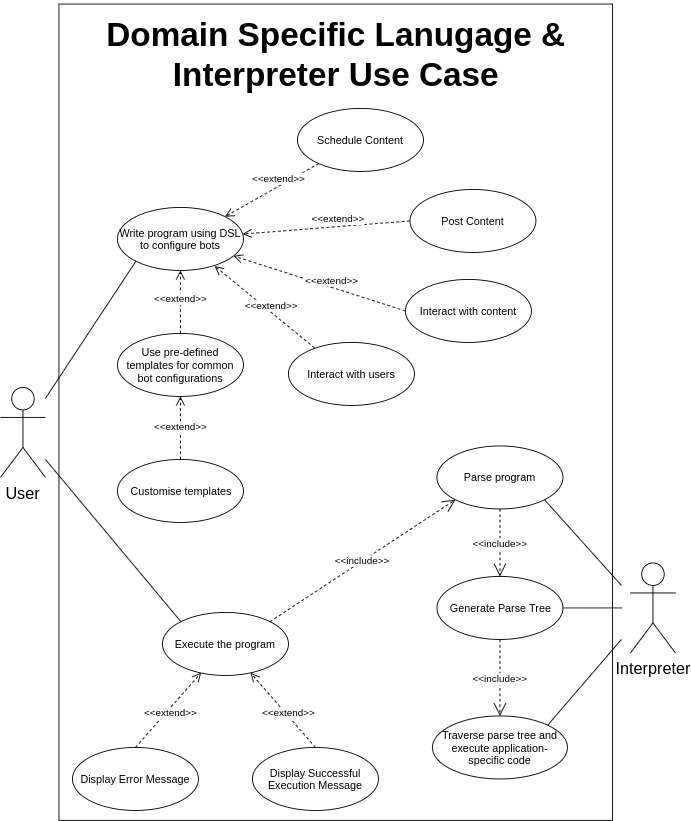
\includegraphics[scale=0.6]{usecasedsl}
 \newline
 \caption{UML Use Case Diagram}
\end{center}

\newpage
\null
\vfill

\begin{center}
 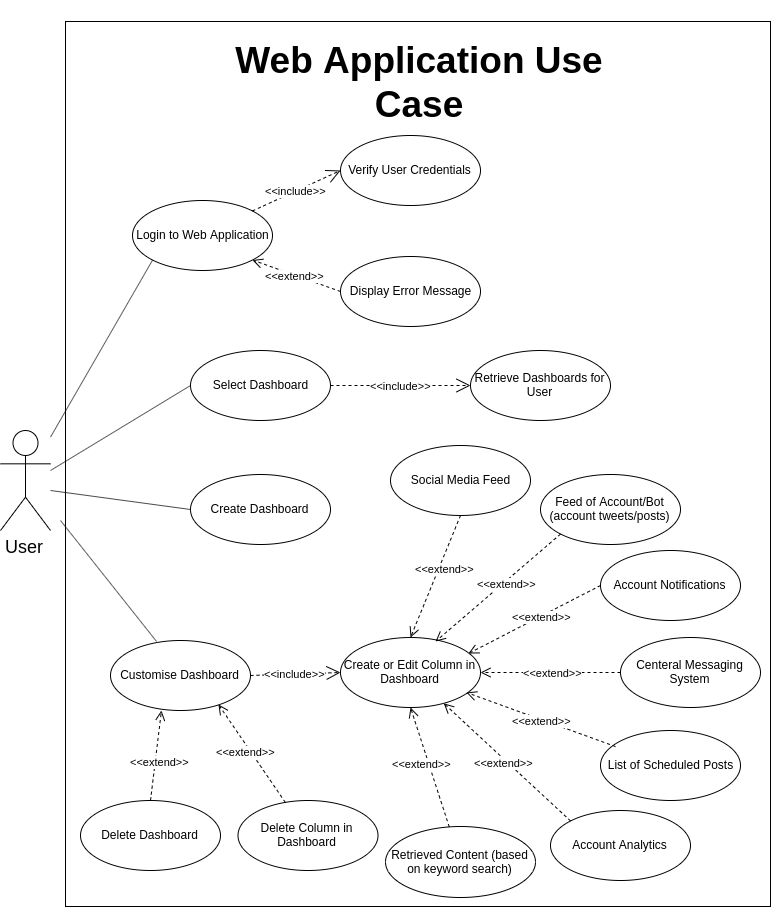
\includegraphics[scale=0.5]{usecasewebapp-2}
 \newline
 \caption{UML Use Case Diagram}
\end{center}

\section{Project Plan}

The project can be split into 5 main tasks. The first main task is the interim report, the next three tasks are three major objectives of the project and the final task is the final report.

\subsection{Task 1: Proposal and Interim Report}

\begin{itemize}
 \setlength\itemsep{-0.75em}
 \item By 10th October 2019, the first draft for the proposal will be completed. The proposal will be finalised with minor potential changes to the smart objectives. 
 \item By 17th October 2019 the proposal will be finalised. This completed document will be approved by the project supervisor and will not change.
 \item By 25th October 2019 the meeting with InCrowd will be completed. This includes a full interview transcript and ethical approval \& consent.
 \item By 8th November 2019 the first draft for the interim report will be completed. The interim report will be finalised with minor potential changes based on supervisor feedback.
 \item By 14th November 2019 the finalised document for the interim report will be completed. This document will be approved by the project supervisor and will be submitted online.
\end{itemize}

\subsection{Task 2: Domain Specific Language}

\subsubsection{Design}

\begin{itemize}
 \setlength\itemsep{-0.75em}
 \item By 14th November 2019, the decisions about what languages, tools and frameworks to be used will be submitted in the interim report.
 \item By 14th November 2019, high level diagrams for how the user will interact with the system and how this reflects the language design will be submitted in the interim report.
\end{itemize}

\subsubsection{Implementation}

The implementation of the Domain Specific Language will be completed in an agile methodology therefore the intricate details of the implementation are not included. What is expected to be completed at deadlines of prototypes, versions and the final system are included.

\begin{itemize}
 \setlength\itemsep{-0.75em}
 \item By 30th January 2020, the first version of the domain specific language will be completed. This prototype will be able to parse an input and generate parse trees based on the grammar of the language.
 \item By 29th February 2020, the second version of the domain specific language and the parser will be completed. This version will be refactored to work with the first version of the interpreter and will likely involve several agile sprints.
 \item By 10th April 2020, the final version of the domain specific language and the parser will be completed. This prototype will include the full language for all functionality of the mandatory functional requirements. This version will be expected to have minor changes and only include bug fixing agile sprints to fix any errors.
 \item By 1st May 2020. the final version of the domain specific language and the parser will be completed. This version will be fully functional and will be the version that is submitted in the final report.
\end{itemize}

\subsubsection{Testing}

The testing for the domain specific language will be completed using unit tests. Git Hook will be used to ensure that unit tests pass when committing to the version control system. Unit tests will be completed during each agile sprint cycle and will thoroughly test the work completed in the cycle.

\begin{itemize}
 \setlength\itemsep{-0.75em}
 \item By 1st May 2020, the unit tests for the domain specific language will be completed. These unit tests will cover all functionality for the final version of the project and testing documentation will be made available in the final report.
\end{itemize}

\subsection{Task 3: Interpreter}

\subsubsection{Design}

\begin{itemize}
 \setlength\itemsep{-0.75em}
 \item By 14th November 2019, the decisions about what languages, tools and frameworks to be used will be submitted in the interim report.
 \item By 30th January 2020, formal designs for the interpreter will be completed.
\end{itemize}

\subsubsection{Implementation}

The implementation of the interpreter will be completed in an agile methodology therefore the intricate details of the implementation are not included. What is expected to be completed at deadlines of prototypes, versions and the final system are included. The development for the interpreter will commence on January 30th after the first prototype of the domain specific language and parser has been completed.

\begin{itemize}
 \setlength\itemsep{-0.75em}
 \item By 14th February 2020 the interpreter will execute the domain specific language and provide the functionality to sign in, tweet, like, follow and retweet on Twitter.
 \item By 29th February 2020 the interpreter will execute the domain specific language and provide the functionality in FR1, FR2 and FR3 in the requirements analysis.
 \item By 10th April 2020 the interpreter will have completed all functionality for the mandatory requirements and as many desirable requirements as possible within this time frame. This version of the interpreter will be expected to have minor changes and only include bug fixing agile sprints to fix any errors.
 \item By 1st May 2020 the final version of the interpreter will be completed. This version will be fully functional and will be the version included in the final report.
\end{itemize}

\subsubsection{Testing}

The testing for the interpreter will be completed using unit tests. Git Hook will be used to ensure that unit tests pass when committing to the version control system. Unit tests will be completed during each agile sprint cycle and will thoroughly test the work completed in the cycle.

\begin{itemize}
\setlength\itemsep{-0.75em}
 \item By 1st May 2020, the unit tests for the interpreter will be completed. These unit tests will cover all functionality for the final version of the project and testing documentation will be made available in the final report.
\end{itemize}

\subsection{Task 4: Web Application}

\subsubsection{Design}

\begin{itemize}
 \setlength\itemsep{-0.75em}
 \item The decisions about what languages, tools and frameworks to be used will be completed by 14th November in the interim report.
 \item By 1st March 2020 formal designs for the UI of the web application will be completed. 
\end{itemize}

\subsubsection{Implementation}

The implementation of the Web Application will be completed in an agile methodology therefore the intricate details of the implementation are not included. What is expected to be completed at deadlines of prototypes, versions and the final system are included. The development for the interpreter will commence on 1st March 2020 after the first prototype of the interpreter has met the initial functional requirements.

\begin{itemize}
 \setlength\itemsep{-0.75em}
 \item By 1st April 2020, the first prototype of the web application will be completed. This will include all mandatory requirements functionality.
 \item By April 10th the web application will have completed all functionality for the mandatory requirements and as many desirable requirements as possible within this time frame. This version of the web application will be expected to have minor changes and only include bug fixing and UI agile sprints to fix any errors.
 \item By 1st May 2020 the final version of the interpreter will be completed. This version will be fully functional and will be the version included in the final report.
\end{itemize}

\subsubsection{Testing}

The testing for the web application will be completed using unit tests. Git Hook will be used to ensure that unit tests pass when committing to the version control system. Unit tests will be completed during each agile sprint cycle and will thoroughly test the work completed in the cycle.

\begin{itemize}
 \setlength\itemsep{-0.75em}
 \item By 1st May 2020, the unit tests for the web application will be completed. These unit tests will cover all functionality for the final version of the project and testing documentation will be made available in the final report.
\end{itemize}

\subsection{Task 5: Final Report}

\begin{itemize}
 \setlength\itemsep{-0.75em}
 \item By 24th April 2020 the first version of the report will be completed. The only changes to this report will be feedback by project supervisor.
 \item By 1st May 2020 the final version of the report will have been completed and this version will be submitted for the project.
\end{itemize}

\subsection{Gantt Chart}

\begin{sidewaysfigure}[h]
    \centering
        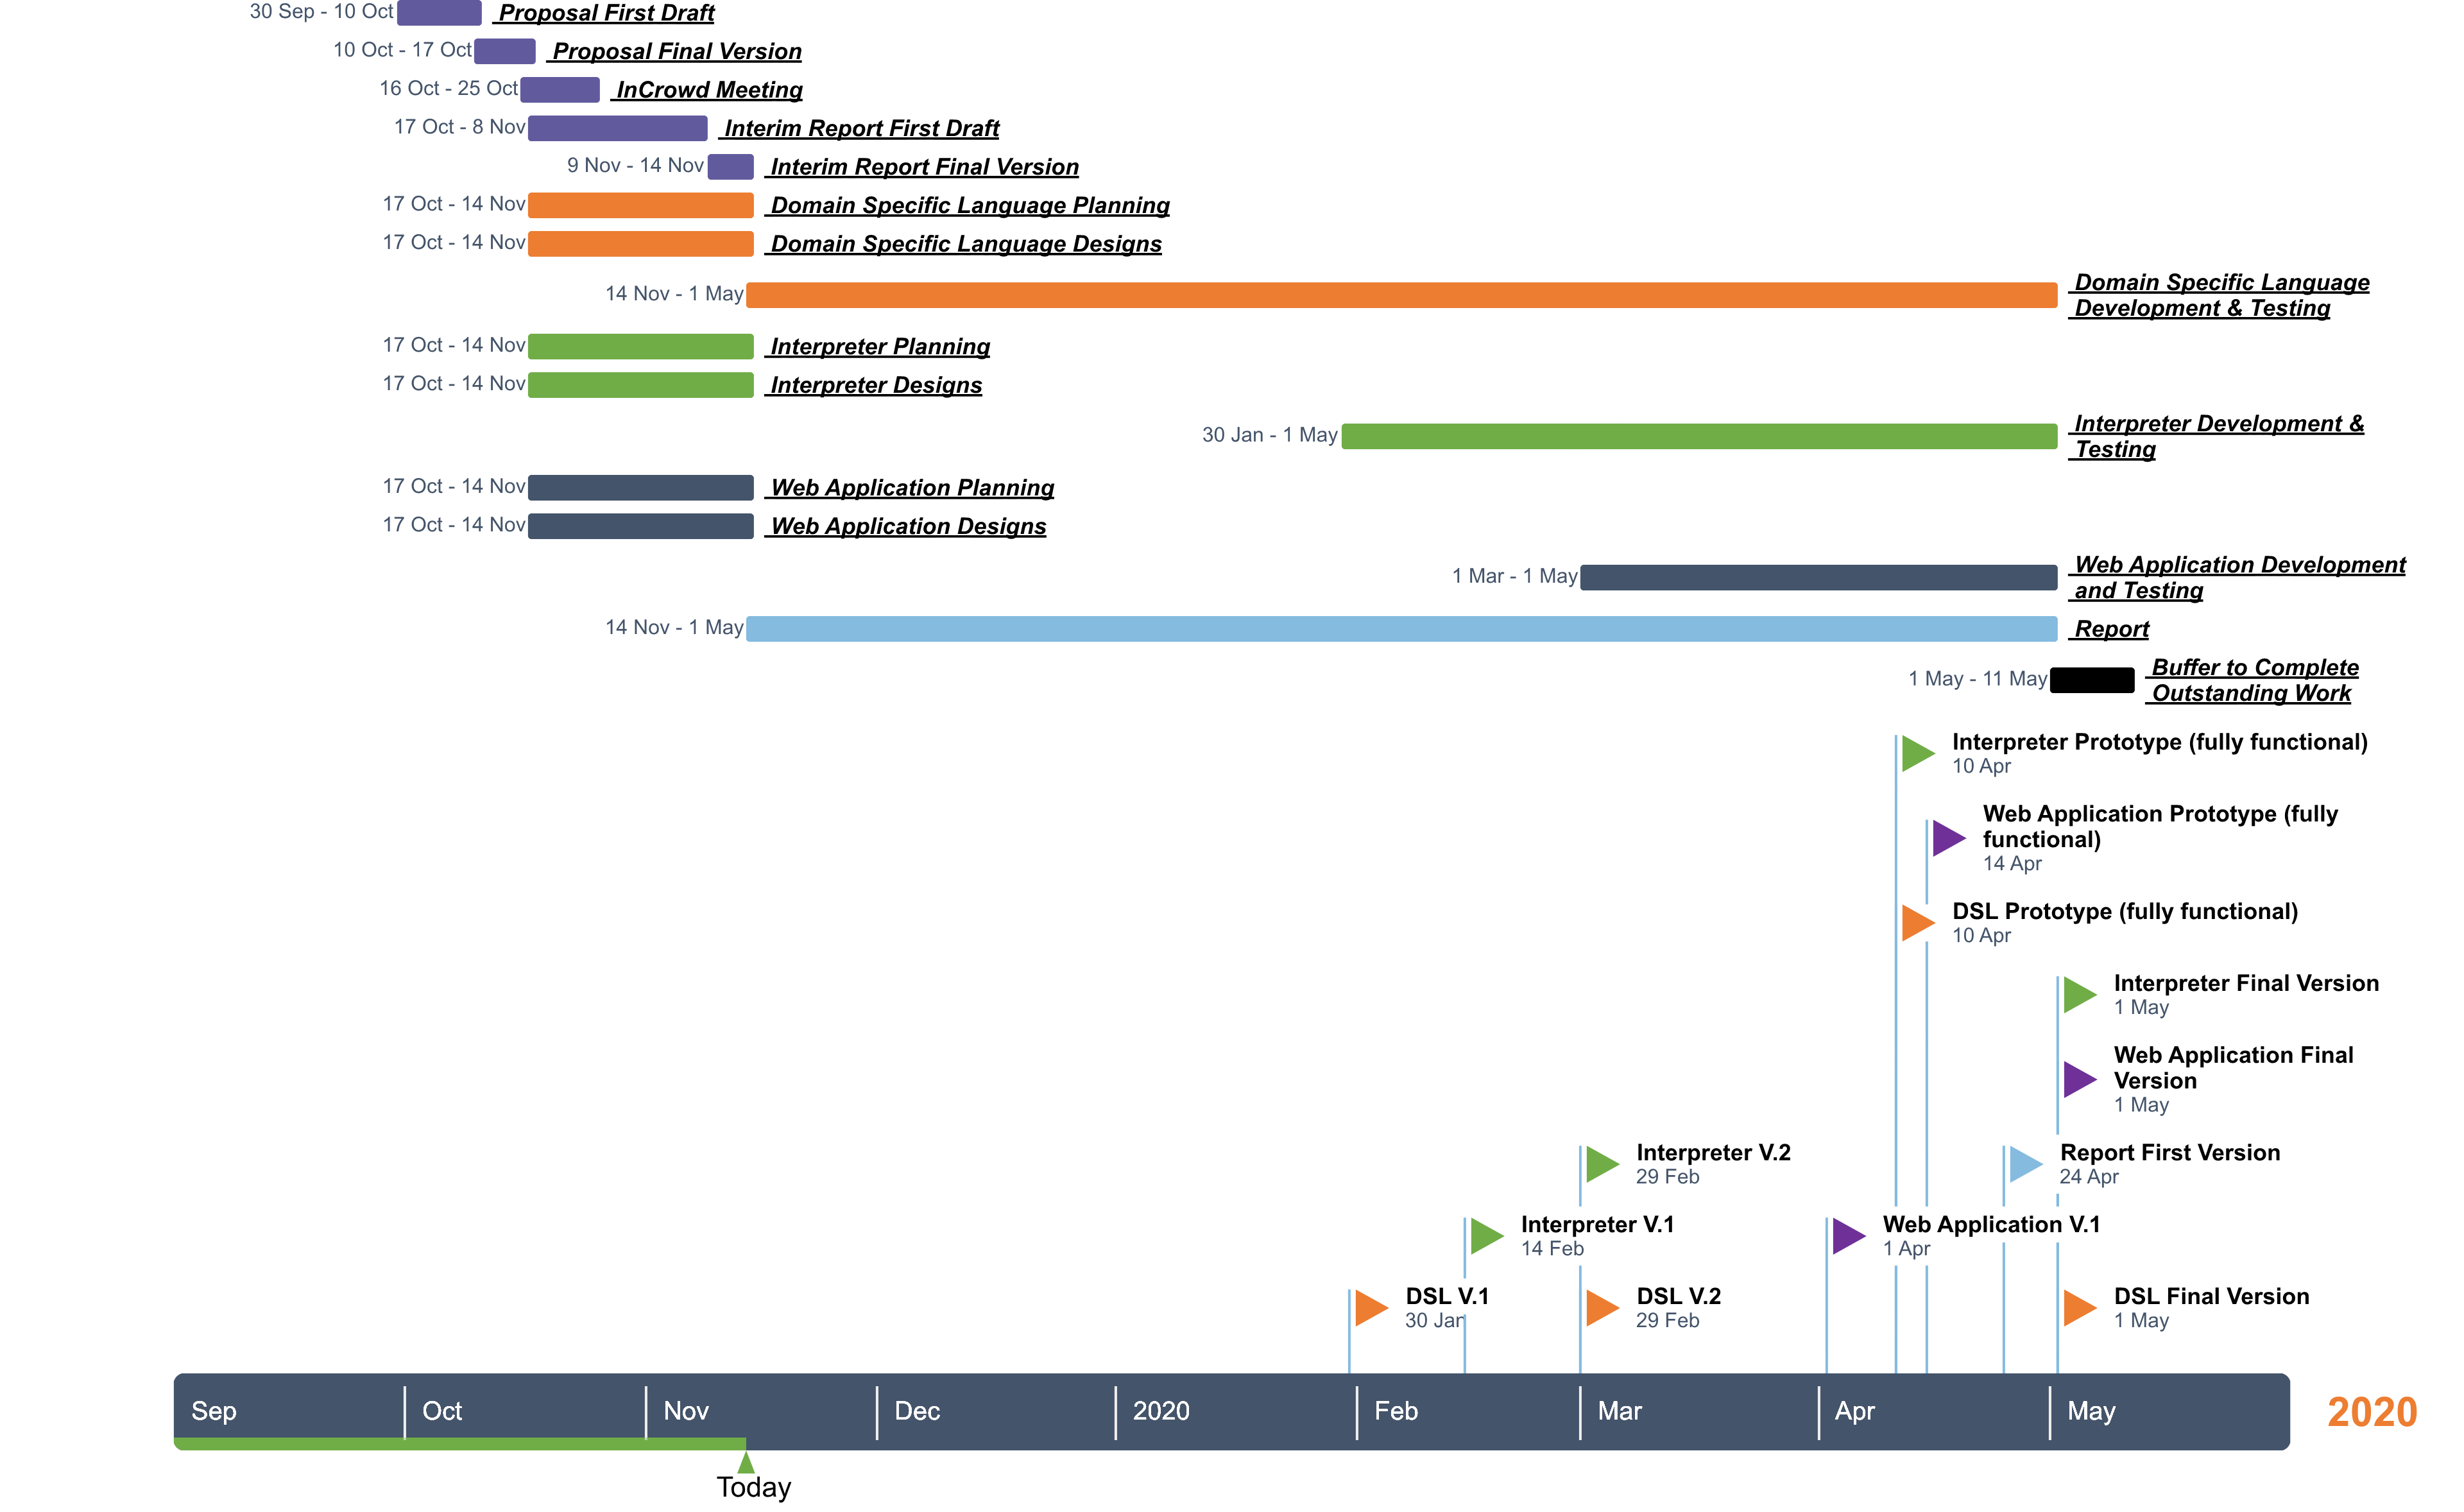
\includegraphics[width=230mm,scale=0.5]{project-outline-2}
        \newline
        \caption{Gantt Chart}
\end{sidewaysfigure}

The Gantt Chart visualises the breakdown of the tasks in a chart. The chart displays the timeline of the overall tasks to be completed and it includes milestones at the bottom to show when each version/prototype of the task should be completed by. The Gantt Chart is currently set to the date the interim report is due, with the interim report, planning and designs already completed.

The tasks are dependent on each other and this has been displayed in chronological order. The domain specific language has to be developed first, the interpreter second and the web application can be developed at any given time. The web application will be developed last as it is not as essential to the project as the domain specific language and the interpreter and the task has a shorter time frame as it is the most competent problem area.


\chapter{Appendix}

\section{Log}

\subsection{Meeting 1: 03/10/2019}

\subsubsection{Agenda}

\begin{itemize}
 \setlength\itemsep{-0.75em}
 \item Discuss next steps and what to do as first meeting.
\end{itemize}

\subsubsection{Discussed Topics}

\begin{itemize}
 \setlength\itemsep{-0.75em}
 \item Proposal: Look at the guide of what to include in the proposal and start working on the proposal
 \item Research: Understand the current market of bots and their functionality and capabilities. Start to research on tools on which you would use.
 \item Meetings: Arrange a meeting with InCrowd sports.
\end{itemize}

\subsubsection{Next Steps}

\begin{itemize}
 \setlength\itemsep{-0.75em}
 \item Work on proposal, arrange meetings and do some general research.
\end{itemize}

\subsection{Meeting 2: 16/10/2019}

\subsubsection{Agenda}

\begin{itemize}
 \setlength\itemsep{-0.75em}
 \item Discuss the research I have completed to gain more scope of the project.
\end{itemize}

\subsubsection{Discussed Topics}

\begin{itemize}
 \setlength\itemsep{-0.75em}
 \item The current stage of research and proposal and what needs to be improved.
 \item What programming languages/frameworks and packages/tool kits which might be helpful for the project.
 \item Recommended books - ANTLR booking for DSL's
\end{itemize}

\subsubsection{Next Steps}

\begin{itemize}
 \setlength\itemsep{-0.75em}
 \item Finalise a date and time to meet with InCrowd.
 \item Email proposal to get feedback.
\end{itemize}


\subsection{Meeting 3: 24/10/2019}

\subsubsection{Agenda}

\begin{itemize}
 \setlength\itemsep{-0.75em}
 \item Discuss the proposal and what can be improved, improve and finalise the questions for InCrowd meeting and discuss the ethics around the interview.
\end{itemize}


\subsubsection{Discussed Topics}

\begin{itemize}
 \setlength\itemsep{-0.75em}
 \item Proposal: Feedback on the proposal and where to improve
 \item Meeting: Finalise meeting questions for InCrowd
 \item Ethics: Ethical guidelines and review for the meeting. Will need consent forms and will need ethical approval if the system is used.
\end{itemize}

\subsubsection{Next Steps}

\begin{itemize}
 \setlength\itemsep{-0.75em}
 \item Start working on the interim report
 \item Arrange meeting after Ian's China trip to get feedback and answer questions about the interim report.
\end{itemize}

\subsection{Meeting 4: 11/11/2019}

\subsubsection{Agenda}

\begin{itemize} 
  \setlength\itemsep{-0.75em}
  \item Introduction
  \begin{itemize}
     \setlength\itemsep{-0.75em}
     \item  How much detail should I go into? Should I aim for it to be easily understandable and then go into enough detail for the reader to understand if they were a final year undergraduate student? 
     \item Do I include aims and objectives in the introduction and Smart objectives?
  \end{itemize}
  \item Professional Considerations
    \begin{itemize}
     \setlength\itemsep{-0.75em}
     \item How much detail should be discussed in regards to the ethics of bots?
     Should examples such as the 2016 US election be discussed?
     \item What do I write about the ethics approval and do I need ethical approval from InCrowd?
    \end{itemize}
  \item Related Work
    \begin{itemize}
     \setlength\itemsep{-0.75em}
     \item How many examples should I include and should I include academic papers?
    \end{itemize}
  \item Requirements Analysis?
    \begin{itemize}
     \setlength\itemsep{-0.75em}
     \item Should high-level diagrams be included?
     \item Should the transcript be included in the appendix?
    \end{itemize}
  \item Log
    \begin{itemize}
     \setlength\itemsep{-0.75em}
     \item Should the log in a minutes format?
    \end{itemize}
  \item Proposal
    \begin{itemize}
     \setlength\itemsep{-0.75em}
     \item Should this be updated to reflect the current scope of the project?
    \end{itemize}
\end{itemize}

\subsubsection{Discussed Topics}

\begin{itemize}
 \setlength\itemsep{-0.75em}
 \item The topics discussed were the different sections to be completed for the
 interim report
    \begin{itemize}
     \setlength\itemsep{-0.75em}
     \item Introduction: The introduction should look at the problem area and introduce your solution to the problem area. Discuss if it is possible to implement a domain specific language for the project and why a programming driven solution might work.
     \item Professional and ethical considerations: Discuss Cambridge Analytica, the risks of automation, how your project could be weaponised and acknowledge the dangers of the project and your solutions to this. You will need consent from Matt and Helen to put in the appendix and may only use selected quotes.
     \item Related Work: Include an academic paper and link the requirements analysis to the related work.
     \item Requirements Analysis: Include high level diagrams.
     \item Log: The log does not need to be converted into minutes format.
     \item Proposal: Update the proposal when necessary.
    \end{itemize}
\end{itemize}

\subsubsection{Next Steps}

\begin{itemize}
 \setlength\itemsep{-0.75em}
 \item Email draft to get feedback.
 \item Arrange meeting for early next week to start project.
\end{itemize}

\newpage

\section{Proposal}

\subsection{Goals}

The goal of this project is to design and implement a domain specific language, a parser and its run time to control the interaction of social media bots with multiple interactive feeds. The DSL will contain the features and capabilities of what a user can do on the social media platforms so they can be automated and scheduled. The goal is for social media marketing teams and individuals to easily automate interactions on the social media platforms and have a web application with a customisable interactive feed for the bots account.

\subsection{Objectives}

The project can be split into three main tasks. This includes:

 \begin{enumerate}
   \item Designing and implementing the domain specific language to produce executable code/commands
   \begin{enumerate}
	   	\item The overall aims of this task are to design and implement the domain specific language. This includes designing and implementing the grammar for the language. The grammar will be used by ANTLR to generate a parser that can build and walk parse trees.
   \end{enumerate}
   \item Implement the interpreter to configure and operate the social media bots
   \begin{enumerate}
	   	\item The overall aims of this task are for the interpreter to use the parse tree to translate it into some efficient intermediate representation and immediately execute this. The interpreter will explicitly execute stored pre-compiled code made by a compiler which is part of the interpreter system. This code will 			interact with the social media API’s to configure and operate the bots.
   \end{enumerate}
   \item Implement an interactive web interface which displays the feeds/interactions for that bot/account
      \begin{enumerate}
	   	\item The overall aims of this task are to create a web application that displays customisable feeds for the social media account that a user can interact with. The web application will require security, multiple user capabilities and web-hooks for the social media API’s to create a personalised feed for the individual user. The interface will be fully customised, which can display all the different feeds for multiple social media accounts on one web application.
   \end{enumerate}
 \end{enumerate}
 
\subsubsection{SMART Objectives for research, planning and interim report}

\begin{itemize}
 \setlength\itemsep{-0.75em}
 \item By October 21st 2019, complete a research document to help with the scope of the project, to understand its potential and identify similar industry technologies.
 \item By October 25th 2019, a meeting will have taken place with InCrowd to discuss their business model, what they would like to see from the project and the current state of the technology and gaps in the market.
 \item By November 14th 2019, the interim report will include GANTT charts, final planning documentation and final designs using high level and low level designs and modelling.
\end{itemize}
 
\subsubsection{SMART Objectives for Task 1}

\begin{itemize}
 \setlength\itemsep{-0.75em}
 \item By November 14th 2019, all designs for the language will have been completed and development will begin.
 \item By January 30th 2020, a first prototype for the domain specific language will be completed.
\end{itemize}

\subsubsection{SMART Objectives for Task 2}

\begin{itemize}
 \setlength\itemsep{-0.75em}
 \item By November 14th 2019, all designs for process of configuring and operating the bot will be completed.
 \item By February 25th 2020, the domain specific language will be able to run and execute commands for social media bots.
 \item By March 9th 2020, the social media bot including the DSL will be completed and finalised. After this point there will no longer be any development dedicated to the Bots.
\end{itemize}

\subsubsection{SMART Objectives for Task 3}

\begin{itemize}
 \setlength\itemsep{-0.75em}
 \item After March 9th 2020, development for the interface and feeds will begin in an agile methodology.
\item By April 13th 2020, the first version of the project will be finalised.
\end{itemize}

 
\subsection{Relevance}
 
The relevance of this project extends to various topics that have been studied at University and covered in previous work experience.

The design and implementation of the domain specific language, parser and interpreter was covered in the Compilers and Computer Architecture module. 

The domain specific language will require rigorous design to ensure that it is scalable, efficient and usable and will require more traditional waterfall planning and techniques. The interface used to display the feeds and interactions of the bots will be developed using Django, which will require an Agile/Scrum methodology. Both these design and development techniques and methodologies are relevant as they were covered in the Software Engineering module, have been used with previous work experience and are widely used in the industry today. 

The programming will be predominately done using Python 3, which I have learnt through the Natural Language Engineering module and I have used in industry. I have also used the Django framework written in Python. 

I have currently not used any API’s in University however I have used some Amazon API’s with previous work experience. 

The primary use of the project is for social marketing teams and individuals to have the ability to automate social media posts and interactions with the posts. I wanted to create something practical and usable and this was all inspired by previous work experience working with paid search marketing teams and tools. The relevance of this project links to previous experience I have and potentially the industry that I would like to work in post University.

\subsection{Resources Required}

No resources required other than access to programming languages, APIs, IDEs, frameworks and packages. All these resources are open source, free or available to use on Software Hub. The resources I that I wish to use are Python 3, ANTLR, Twitter API, Facebook API, Instagram API, Git and Github, Django (Python Web Framework), \LaTeX, Clubhouse and Intellij. I plan to do all development on my laptop running Ubuntu 18.04 LTS.

\newpage

\section{Ethical Consent}

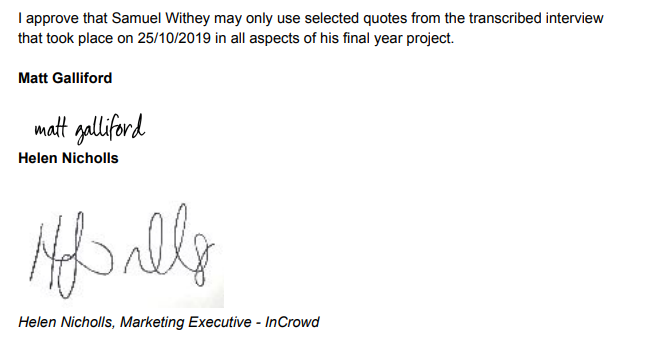
\includegraphics[scale=0.5]{ethical-approval}

\bibliography{references}
\bibliographystyle{plain}

\end{document}